\section{Task title}

\begin{table}[]
   \centering
   \begin{tabular}{l|l}
   Parameter             & Value \\ \hline
   Focal Length X (px)   & 4550  \\ \hline
   Focal Length Y (px)   & 4580  \\ \hline
   Principal Point X (px) & 2930  \\ \hline
   Principal Point Y (px) & 1968  \\ \hline
   Skew                  & 0    
   \end{tabular}
   \caption{Intrinsic Parameters}
   \label{params:table}
\end{table}

\paragraph{Using} MATLAB's camera calibration app we were able to find the intrinsic parameters of our camera. The app takes as input a series of images with a calibration grid visible in the image, it then uses the intersections of the grid as correspondences across all the images thus allowing to the estimate the parameters. All the values, as shown in \autoref{params:table}, are reported in pixel measurements. This could be because it is easier for other MATLAB methods, which use the camera parameter, to operate using pixel lengths. Regardless, the raw values are reported here. Supposedly, these values were very accurate with MATLAB reporting an average error of approximately 1.8\% for the focal length and 1.4\% for the principal point. 

\autoref{distortion:img} is a vector field of how MATLAB would undistort an image based on the camera calibration we performed. As you can see it take the outermost pixels and spread the further apart. This suggests that the camera distorts the image by compacting the edges, this is also known as barrel distortion. The amount of distortion in the camera isn't very high but that is to be expected of modern photography tools.

\begin{figure}[ht]
   \centering
   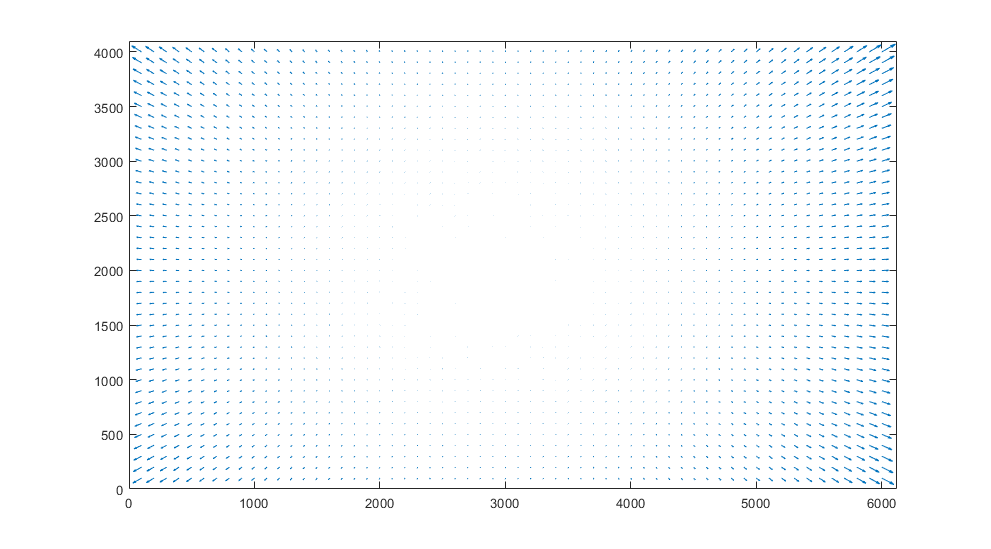
\includegraphics[width=0.8\linewidth]{Task3/images/distortion.png}
   \caption{Estimated Camera Distortion}
   \label{distortion:img}
\end{figure}